\chapter{Machine learning approach}
\label{ch:MachineLearning}
\graphicspath{{Chapter4/Chapter4Figures/}}
The previous chapter briefly described the basic workings of the optical mark recognition (OMR) system inside the automatic test grader. There is still one critical piece of evidence that has not yet been observed in this basic system. This information is the characters that the student writes in the designated boxes.

\nomenclature[A]{$DCNN$}{Deep convolutional neural network}
This next chapter will provide two machine learning approaches to significantly improve the accuracy in identifying digits over the previous standalone basic system, discussed in Chapter \ref{ch:ImageProcessing}. An approach to locate and classify hand written characters, provided by the students, using a deep convolutional neural network (DCNN), is described. Next a more accurate method in determining the true digit, student answers and student number, using probabilistic  graphical models (PGM), is discussed. This PGM method is found to be accurate enough to determine the student number by only using the character recognition information provided.

\section{Character recognition using a neural network}

\subsection{Summary}

This section focusses on processing the characters that the students write down in the designated boxes, as shown in Figure \ref{fig:sa}. To process these digits a machine learning approach, called a neural network, is implemented. Once the test sheet is processed all the character digits can be found. A 28 by 28 digit image is then created for each character found on the page.
\begin{figure}
  \centering
  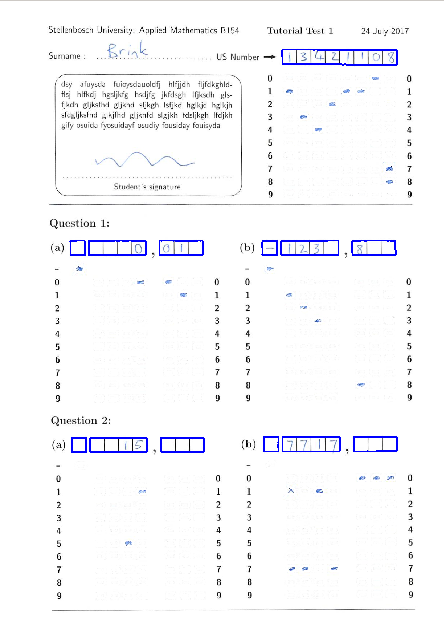
\includegraphics[width=6cm]{DigitScan}\\
  \caption{Image showing found contours for boxes used for character recognition.}
  \label{fig:sa}
\end{figure}

A neural network then processes these digit images and produces an estimate to what digits are most likely to be present in each image.

\subsection{Preprocessing to find individual digit image}
\label{sec:preprocess}

Before each digit can be classified using a neural network, the individual 28 by 28 pixel digits must first be found inside the test sheet. To do this image processing is required. This is done in 6 steps as seen below:

\begin{enumerate}
\item Find the contour closest to the expected location of the block, calculated in Section \ref{sec:findTemplate}. This is ilustrated in Figure \ref{fig:sa}. It can be seen that the bubbles are already processed.

\item Transform the image to become fully rectangular using OpenCv's $four\_point\_transform$ method. This method applies a four point perspective transform on the image to reshape it into a rectangular form. An example of the final product can be seen in Figure \ref{fig:bp}.

\begin{figure}
  \centering
  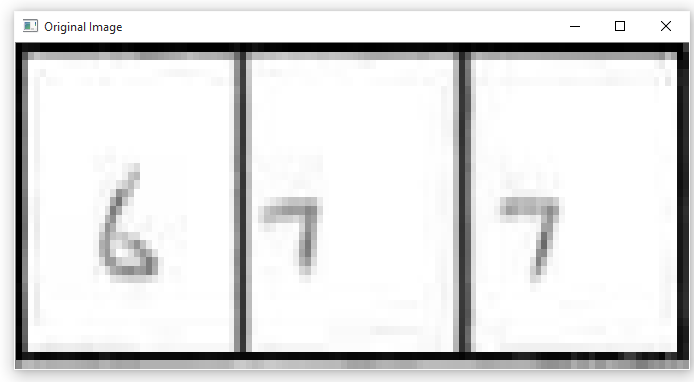
\includegraphics[width=7cm]{BeforeProcessing}\\
  \caption{The box contour found is normalized to form a rectangular shape.}
  \label{fig:bp}
\end{figure}

\item Perform a Radon transform on the image, at an angle of 0$^{\circ}$ and 90$^{\circ}$ to find the dark lines in the blocks. These lines are the removed from the image, as seen in Figure \ref{fig:ar}. The mathematics behind a Radon transform is described in Section \ref{sec:RadonTransform}.

\begin{figure}
  \centering
  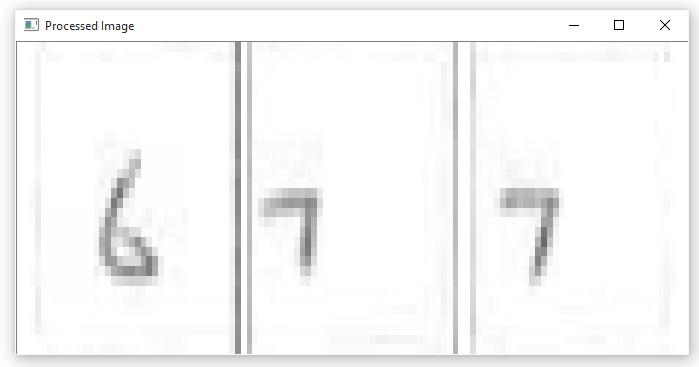
\includegraphics[width=7cm]{AfterRadon}\\
  \caption{Box after black lines gets filtered out, found using a Radon transform.}
  \label{fig:ar}
\end{figure}

\item Use the values received from the Radon transform to segment the image into the different boxes.
\item Using a custom segmentation algorithm to find the pixels most likely to belong to the digit. This algorithm is developed and implemented using breath first search technique to cluster the image into different segments. The algorithm works by first searching the image for pixels higher that a threshold value. This value specifies if an pixel is background or belongs to an image segment. Then all the pixels higher that the threshold value gets assigned to a segment. A segment is thus classified as a local region that does not connect to any other segment through pixels higher that a threshold. The segment that most likely represents the digit is then extracted, as seen in Figure \ref{fig:c}.
\begin{figure}
  \centering
  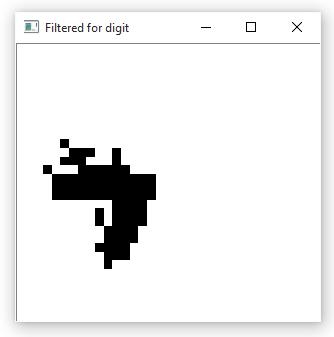
\includegraphics[width=3cm]{Cluster}\\
  \caption{Custom segmentation algorithm used to find the main cluster in the remaining image.}
  \label{fig:c}
\end{figure}

\item The area that the segment occupies then gets calculated, as seen in Figure \ref{fig:areaLoc}

\begin{figure}
  \centering
  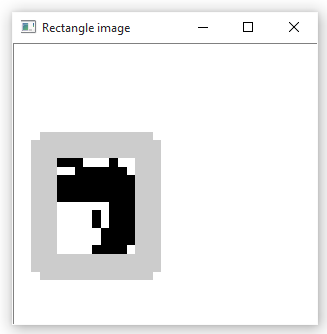
\includegraphics[width=3cm]{DetectArea}\\
  \caption{Area block drawn around segment most probable to belong to the digit.}
  \label{fig:areaLoc}
\end{figure}

\item Next the image is centred and normalized using the image area as reference. This is seen in Figure \ref{fig:final}

\begin{figure}
  \centering
  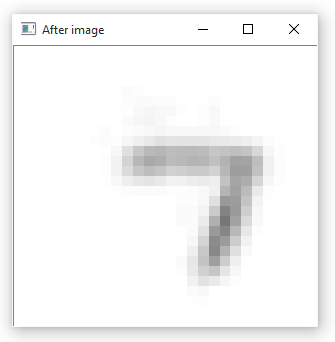
\includegraphics[width=3cm]{TranslateAndScale}\\
  \caption{Image after final translation and normalization is applied.}
  \label{fig:final}
\end{figure}

\item The image is then reshaped into a 28 by 28 greyscalled image to be processed by the neural network.
\end{enumerate}

Each digit on the test sheet is now separated and can be used as input to an neural network. An overview of this neural network will be given next.

\subsection{Neural Network Classification}

\subsubsection{Introduction}
A neural network is a powerful machine learning tool for approximating complex functions. The basic architecture of a neural network can be seen in Figure \ref{fig:nn}. A Deep Convolutional Neural Network(ANN) consist of an input, hidden and output layer, as described in \citet{MichealN2015}. A neural network is a simplified approximation of how neurons in the brain works. Each neuron in the network acts as a small processing unit. With a initial input, an output is determined by measuring the last output node, as shown in the figure. The output can only be determined once each layer have been calculated one after the other.

\begin{figure}
  \centering
  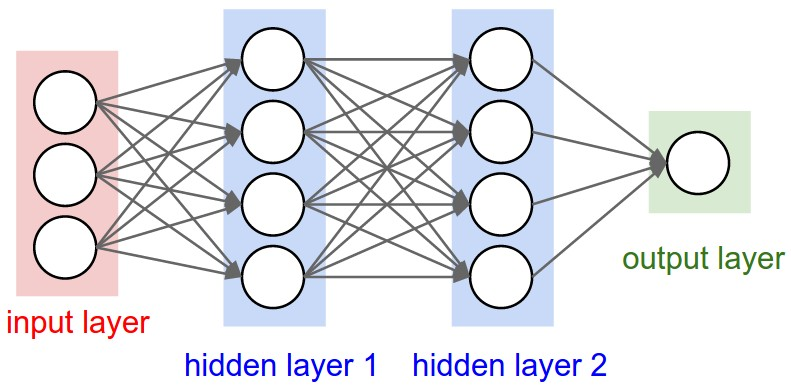
\includegraphics[width=10cm]{NN}\\
  \caption{Basic structure of a neural network, from \citet{karpathy2017}}%, 
  \label{fig:nn}
\end{figure}

For this project, a neural network is trained to estimate the probability of which of the 10 digits, from 0 to 9, are most likely present in the input image. The neural network will take a 2 dimensional array, representing a greyscaled image, as input to the network. Figure \ref{fig:mnist} illustrates an example input of a neural network using and 14 by 14 example image. 

\begin{figure}
  \centering
  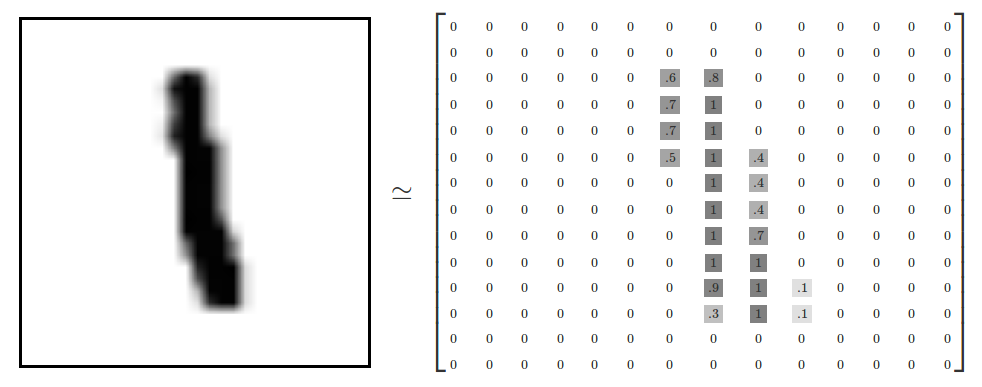
\includegraphics[width=10cm]{MNIST}\\
  \caption{Example image used as input to the neural network, from \citet{tensor2017}}
  \label{fig:mnist}
\end{figure}

For this project a 28 by 28 greyscalled image is used as input. Thus if each pixel represents one value, ranging from 0.0 to 1.0, there is total of 748 input values. The basic workings of a neural network is described in the next section.


\subsubsection{The artificial neuron}
The neuron unit is the small processing unit used to build a neural network. The first step in calculating the output of a neural network is to find the weighted sum of the inputs. All the variables in this network are floating point values. A bias variable is added to allow a neuron to have an possible offset on its output. The weighted sum of these inputs are added with a bias variable to give,
\nomenclature[S]{$x_{i}$}{Input value at index i.}
\nomenclature[S]{$w_{i}$}{Weight value at index i.}
\nomenclature[S]{$b$}{Bias variable added to allow a neuron to have an offset in its output.}
\nomenclature[S]{$z$}{Weighted some of a neuron's inputs and internal variables.}
\nomenclature[S]{$c$}{Number of inputs to a neuron.}
\begin{align}
% \nonumber to remove numbering (before each equation)
  z =  &\displaystyle{\sum_{i=0}^{c} x_{i}*w_{i} + b}.
\label{eqn:nnOut}
\end{align}
Where $c$ is the number of inputs. $x_{i}$ and $w_{i}$ respectively are the input and weight values at index i. $b$ is a is term that enables and offset in the output($z$) of the neuron.
The summed value then gets normalize using an sigmoid function, seen seen
\nomenclature[S]{$\sigma(z)$}{Normalization function in a neural network.}
\begin{align}
  \sigma(z) =  &\displaystyle{\frac{1}{1 + e^{-z}}}.
\label{eqn:sigmoid}
\end{align}
This artificial neuron thus takes in a weighted input with a bais and produces a normalized output $\sigma(z)$. By adjusting the weights and bais variable, each neuron can learn to exhibit certain characteristics. This process thus allows different functions to be approximated by adjusting these variables. If a network of these neurons is used together, as shown in Figure \ref{fig:nn}, complex functions can be trained onto the network. In this project these weights and biases needs to be set to specific values, to allow the network to accurately categorize digits from an image. To do this these weights and biases will be trained form training data, as seen in Section \ref{sec:trainNN}.

\subsubsection{Generating output from an neural network}
After the 748 input values have been assigned to the network inputs, each of the network's layers can be calculated consecutively one after another. The first hidden layer will thus use the 748 input values and produce a normalize output for each of the neurons in that layer. This is done using the previously mentioned Equations \ref{eqn:nnOut} and \ref{eqn:sigmoid}. Once the first layers's outputs are calculated the next layer can be calculated. This process is repeated until all the layers are calculated in the hidden section. The output layer is then calculated using the same method. For the character recognition in the test grader, 10 output neurons are used, corresponding to the probability of the 10 digits being present. The values observed on the output neurons, gets normalized and used as the probability of each digit being present, using
\begin{align}
  p(i) =  &\displaystyle{\frac{\sigma(z_{i})}{\sum_{k=0}^{10} \sigma(z_{k})}}.
\label{eqn:normal}
\end{align}
Where $p(i)$ is the probability of digit $i$ being the character in the image. The value $\sigma(z_{i})$ is the output of the output neuron at index $i$.
%For a more detailed explanation on the DCNN used in this project, refer to Appendix \ref{sec:DCNN}. (Maak dit dalk dat die neural network in overview hier beskryf word. Soos hoe dit werk as a black box. En dan Verder word die wiskunde agter NN and DCNN agter in die appedix beskryf)
%Bv: For a mathematical description on neural networks and DCNN, refere to Appendix \ref{sec:DCNN}.
\subsubsection{Training of neural network}
\label{sec:trainNN}
To train a neural network the MNIST dataset is used. This is a database that has a labelled training set of 60,000 images, and a labelled test set of 10,000 images. Each image has an accompanied label that specifies what digit is in the picture. The neural network is trained by using this training set to adjust its internal weights and bias variables so that the network's output better represent the labelled training data. The basic idea behind the training method used in a neural network is described in the following steps. For a more detailed description refer to Appendix \ref{ap:Algorithms}.

\begin{enumerate}
\item Calculate the network's output for each of the training images used in this training round.
\item Get the error function of the network, using a formula that compares the true label of the training image, with the estimated label of the network.
\item Calculate the value with which each weight should be changed to reduce the error function slightly. One method of doing this is using gradient decent with back propagation.
\item Repeat steps 1-3 until a time or accuracy criteria is met.
\end{enumerate}
\section{Probabilistic Graphical Models}
\label{sec:PGM}

The final step in determining the students answers is to probabilistically determining the most likely answers, given the bubble and character evidence presented. To do this 3 probabilistic graphical models (PGM) are implemented.

\subsection{Overview}
For this project a graphical approach is followed in representing the software developed. A graphical model in essence allows software to be represented as information (nodes or circles) and relationships (directed arrows). The directions of the arrows represents what information causes other information to be created, thus given a parent to offspring interpretation). An example of such a graph can again be seen in Figure \ref{fig:pgmDigit}. These graphs allows for intuitive reasoning about how the system should operate. For this project an observation is made in the form of an image which is used as evidence. The system is then tasked with predicting what the written entries are given this information. Due to the probabilistic nature of the system a probabilistic component is also needed in this graphical models. Thus a probabilistic graphical model (PGM) is used.

A probabilistic graphical model (PGM) is a probabilistic graph containing random variables, where the graph expresses the conditional independence structure between these variables. The type of PGM used for this project is a Bayesian network. A Bayesian network models a set of random variables and their conditional dependencies via a directed acyclic graph (DAG). As seen in Figure \ref{fig:pgmDigit}, arrows are used to indicate which variables are conditionally dependent on others. 

\subsection{Intended digit model}

\subsubsection{Structure of the graph}


\begin{figure}
  \centering
  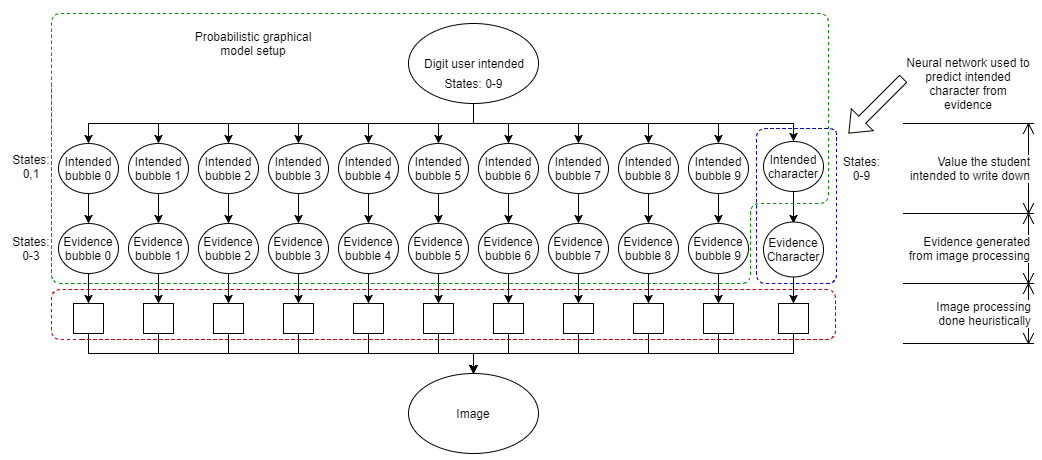
\includegraphics[width=16cm]{pgmDigit}\\
  \caption{Graphical setup for determining the intended digit written by a student.}
  \label{fig:pgmDigit}
\end{figure}


The figure should be interpreted in the direction which information flows. Originally a student has a certain digit that he/she wants to portray on the page. This is given by the 'Digit user intended bubble'. There are 10 possible digits to consider and thus the bubble has 10 possible states. The intended digit gives rise to the intended bubbles and character that the student wants to write down. The student might sometimes mistakenly think that the first bubble represents 0 and thus even if the intended digit is 0 the intended bubble might be 1. Thus, this must also be done in a probabilistic manner to compensate for this uncertainty. The intended bubbles and character then produces evidence, as seen in Figure \ref{fig:pgmDigit}.  

\begin{figure}
  \centering
  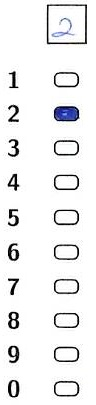
\includegraphics[width=1cm]{column}\\
  \caption{Column with the evidence that gets considered for the calculation of an intended digit.}
  \label{fig:column}
\end{figure}

When looking at Figure \ref{fig:column}, it is observed that there are 11 evidence areas to consider. They are the the 10 bubbles and the character block. The process of writing down this digit introduces so noise into the system, due to the fact the student is not always going to write down the digit in exactly the same way. Thus the evidence is also probabilistically linked to the 'intended bubble' and 'intended character' parent distribution. This evidence then gets written down on the paper and is what ultimately influences how the image looks. Each of the bubbles can take one of 4 states as evidence. These states are blank, crossed-out, partially coloured in and fully coloured in. The character block evidence is a 28 by 28 greyscale image. Thus it can have 28*28*256 possible states, where 256 is the possible pixel intensities of each pixel. This value with true range 0 to 256, gets converted into a normalized value between 0.0 and 1.0 before it gets assigned as inputs to the neural network.


\subsubsection{Estimating the intended digit}
\label{sec:intendedDigit}
After the model is constructed the intended digit needs to be estimated, with the image as evidence. This can be done by reasoning from the bottom (image evidence) upwards to the intended digit. The first step is to process the image, using of image processing, to produce more tractable evidence. Producing the bubble evidence from the image is described in Chapter \ref{ch:ImageProcessing}. In Section \ref{sec:preprocess}, the process to extract the character evidence from the image is also described. Using the neural network the probability of intended character, given the character box, can be determined. After these steps is completed the intended digit can be estimated using the PGM. This is done by first setting the evidence node to the values calculated when image processing were done on them. The 'intended character' node then gets set to prior calculated through the use of the neural network. After this is done inference is done on the PGM and the resulting probability of each digit is calculated for the 'intended digit node'. The PGM structure can again be seen in Figure \ref{fig:pgmDigit}. 


\subsection{Intended answer model}
\label{sec:pgmStudentNum}

\subsubsection{Structure of the graph}

There are 8 possible columns to use for an answer. The first column represents the sign of an answer. Thus two signs are possible. For each of the remaining 7 columns a number from 0 - 9 can be represented. Thus there are ten possible values for each column. This gives a possible number of values that a answer can take to be $2*10^7 = 20 000 000$. Each of these states needs to be calculated and becomes computationally intractable. Thus a assumption is needed to reduce the number of possible states. A fair assumption to make, is that all $20 000 000$ possible values are equally likely to be written down. Thus each column digit becomes independent of the another columns values. This means that if a value in one column is known, it does not influence the probabilities of the other columns being a certain value. Thus the number of states to calculate now becomes $2+10*7=72$, because each column's states can now be calculated independently. Thus knowing this independent property the answer model can be described as a combination of 7 digit models with a heuristic calculation of the intended sign. This model is illustrated in Figure \ref{fig:stdAns}.

\begin{figure}
  \centering
  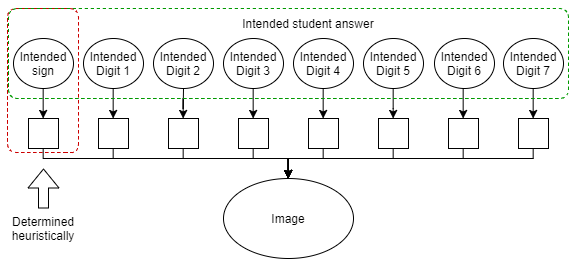
\includegraphics[width=10cm]{ans}\\
  \caption{Graphical setup of determining student answer.}
  \label{fig:stdAns}
\end{figure}


\subsubsection{Estimating the intended answer}
\label{sec:intendedDigit}

In the previous section it was found that determining the intended sign and digit for each column the intended answer can be found. Thus the intended digit for each column is calculated separately using the digit model, as described in Section \ref{sec:intendedDigit}. The intended sign is determined heuristically by using the image processing methods described in Chapter \ref{ch:ImageProcessing} to find if the bubble underneath the sign is coloured in. Once this is done the intended answer is determined by combining the estimated sign and digits in the order seen in Figure \ref{fig:stdAns}.

\subsection{Student number model}
\label{sec:pgmStudentNum}

\subsubsection{Structure of the graph}

For a student number additional information is present. Knowing the digit value of one column changes the probability of each other column taking a certain value. The reason for this is, because there is only a limit number of student numbers to consider. Thus if the first digit is a 2, only student numbers starting with 2 still have to be considered. To account for this fact an additional node is added above the individual digit probabilities. This node represents the probability of each student number being present in the image and is related to the intended digits. The student number thus produces the intended digits. This node will have $+- 900$ states, depending on the number of student numbers. The student number graph can be seen in Figure \ref{fig:stdNum}.

\subsubsection{Estimating the student number}

Now that the graph has been setup the model can be used to infer the most probable student number. By setting all the bubble evidence and character priors the student number probabilities can be inferred. This model allows for a accurate result, because most student numbers are quite different to one another. It is found that if the student provides only character information and no bubbles are coloured in, the student number can still be estimated reliably. These results is states in Section \ref{ch:Results}.

\subsection{Training the model}

For this project the conditional probabilities for the intended digit model was found by using training data. From these distributions the answer model can also be constructed due to it only consisting of independent digit models. The probability of a student number given the intended digits was estimated manually.

As seen in Figure \ref{fig:pgmDigit},the digit PGM will include the bubble evidence as well as a prior probability which the neural network provides. Once these values are assigned, the PGM model will infer the intended digit using the conditional probability distributions specified. To do this the conditional probabilities of the PGM, must first be determined from data.



The process of training a PGM is a simple process once enough training set is present. This was done by allowing the initial software, without the PGM model, classify the digits. Thus the training set contains the bubble and neural network outputs as evidence. The training set then also includes the intended bubbles and intended digit, as estimated by the image processing unit. Once all these test data are gathered, the conditional probabilities can be calculated. These probabilities then gets stored and used as prior probabilities in the PGM.

\section{Conclusion}

This chapter looked at two machine learning techniques to improve the accuracy with with the system infers the answers written on each scanned test sheet. A method was shown, using a neural network, to estimate the probability of each digit given only the character box as input. Additionally a approach was discussed, using a PGM, to allow the system to make a final prediction of what the student intended to write down given the bubble and character boxes as evidence.

The following chapter will cover the validation and results of the system from weekly grading done for the Applied mathematics department.